\chapter{Introducción}\label{ch:introduccion}
\thispagestyle{empty}

\vspace{50pt}

\begin{adjustwidth}{50pt}{50pt}
    Este capítulo contextualiza las problemáticas que motivan los estudios
    que se realizan en esta tesis. Se presentan los temas de la energía, el 
    transporte y el litio, donde se mencionan distintas proyecciones para el 
    futuro de los vehículos eléctricos y la demanda de litio impulsada por 
    los mismos. También se introducen aspectos relevantes de las baterías de
    ion-litio comerciales y las que se encuentran en etapa de investigación.
    Por último se concluye con los objetivos y la estructura de la tesis.
\end{adjustwidth}

\clearpage
\newpage
\thispagestyle{empty}
\mbox{}
\newpage

% Copyright (c) 2024, Francisco Fernandez
% License: CC BY-SA 4.0
%   https://github.com/fernandezfran/thesis/blob/main/LICENSE
\section{Contextualización}

El calentamiento global aparece como el mayor problema ambiental de este siglo.
El mismo se refiere al aumento de la temperatura media de la atmósfera y por 
ende a sus consecuencias en  el clima. Esto es debido al efecto que producen 
las actividades humanas, 
como por ejemplo la quema de combustibles fósiles, que emite 
a la atmósfera grandes cantidades de CO$_2$, entre otros gases de efecto 
invernadero, o la deforestación. Estos gases absorben la radiación infrarroja emitida por la tierra y la reemiten, 
provocando un incremento de la temperatura de la misma que lleva asociado un 
aumento en la frecuencia y la intensidad de eventos climáticos extremos. %\cite{houghton2005}. 
De acuerdo a el Panel Intergubernamental del Cambio Climático 
\cite{IPCC}, desde la época preindustrial, las actividades humanas han provocado 
aproximadamente 1.0$^{\circ}$C de calentamiento global y al ritmo actual se van 
a sobrepasar los 1.5$^{\circ}$C antes del 2050, un cambio en la temperatura
media que las medidas previas al aumento de las actividades mencionadas no habían llegado a alcanzar. Limitar el 
calentamiento a esta temperatura requiere que se realicen rápidamente cambios 
sin precedentes en la tecnología y en el comportamiento humano. Uno de los 
cambios más importante es el de la matriz energética, en la cual las energías 
renovables deberán suministrar alrededor del 80\% de la energía para 2050, donde 
los vectores energéticos, como las baterías de litio, juegan un rol fundamental 
debido a la intermitencia de estas formas de generación de energía.

El litio es el metal más liviano de la tabla periódica y uno de los elementos más
importantes dentro de los minerales necesarios en la producción de baterías de
litio. En particular, para la Argentina tiene un interés económico, social, 
industrial y tecnológico ya que es uno de los países que integran, junto a 
Bolivia y Chile, el Triangulo de Litio, el cual acumula el 70\% de las reservas 
mundiales de fácil extracción de este mineral. Esto último debido a que esta cantidad de reservas
se encuentran en salares de los que, a grandes rasgos, es más barato
extraer litio de ellos en comparación a las rocas de las cuales se puede extraer 
litio en una míneria usual, como las pegmatitas. A pesar de esto se tienen que
llevar a cabo distintas consideraciones ambientales, sociales y legales del 
proceso de extracción e incentivar el desarrollo de valor agregado a dicha 
extracción \cite{gutierrez2022, petavratzi2022, obaya2021, romero2021, 
heredia2020, fornillo2019}.

En esta tesis se presentan estudios computacionales sobre materiales para el 
desarrollo de electrodos de baterías de ion-litio de próxima generación. Se 
abordan dos perspectivas, una con el objetivo de tener baterías que frente a una 
carga rápida retengan un porcentaje considerable de la capacidad y otra 
utilizando electrodos que permitan almacenar mayor cantidad de energía que los 
actuales.


\section{Energía, transporte y litio}

En la actualidad se utilizan distintas formas para generar energía y pueden 
dividirse en dos grandes tipos, las renovables y las no-renovables. Estas últimas
dominan la producción de energía mundial y están compuestas principalmente por 
combustibles fósiles y centrales nucleares, mientras que las energías renovables
abarcan más variantes como la biomasa, la hidráulica, la eólica y la solar, pero 
aún no son lo suficientemente utilizadas. Una de las particularidades de estas 
fuentes de energías renovables es su producción intermitente mientras que el 
consumo de la misma, independientemente de cómo se genere, es a demanda. Esto 
hace que sea necesario el involucramiento de vectores energéticos que permitan 
almacenar y transportar el excedente de energía que se genera en sus períodos de 
mayor producción para luego ser utilizada en los momentos de mayor demanda.

El sector del transporte terrestre, marítimo y aéreo es responsable de más de un 
tercio de las emisiones de CO$_2$ debido a su dependencia en los combustibles 
fósiles \cite{IEA}. Dicho esto, está claro que se debe fomentar opciones de desplazamiento menos intensivas
en carbono y con tecnologías más eficientes, como los vehículos eléctricos (EVs),
cuyos motores poseen una eficiencia para convertir la energía eléctrica en energía para las ruedas que ronda el 80\%, compárese este valor con las
eficiencias entre el 12\% y el 30\% de los motores a combustión interna para la misma tarea \cite{DOE}.

En los últimos años se ha producido un crecimiento exponencial en las ventas 
anuales de los EVs, como puede observarse en la Figura \ref{fig:evs}a \cite{EVV}. En la
última década, dichas ventas aumentaron aproximadamente un 500\% y se estima que
para la próxima década las ventas se multipliquen por 10. Estas ventas están 
concentradas en China y en algunos países y estados de Europa y Estados Unidos, 
respectivamente, debido a que en los países en desarrollo y emergentes influye 
negativamente su costo alto de adquisición y una falta de infraestructura para la 
recarga de sus baterías. En particular, durante el 2022 en Noruega el 79.3\% de 
los automóviles patentados fueron eléctricos. En el país que le sigue en la lista,
Suecia, se patentó un 32.1\% de EVs en dicho año \cite{PWC}.
\begin{figure}[h!]
    \centering
    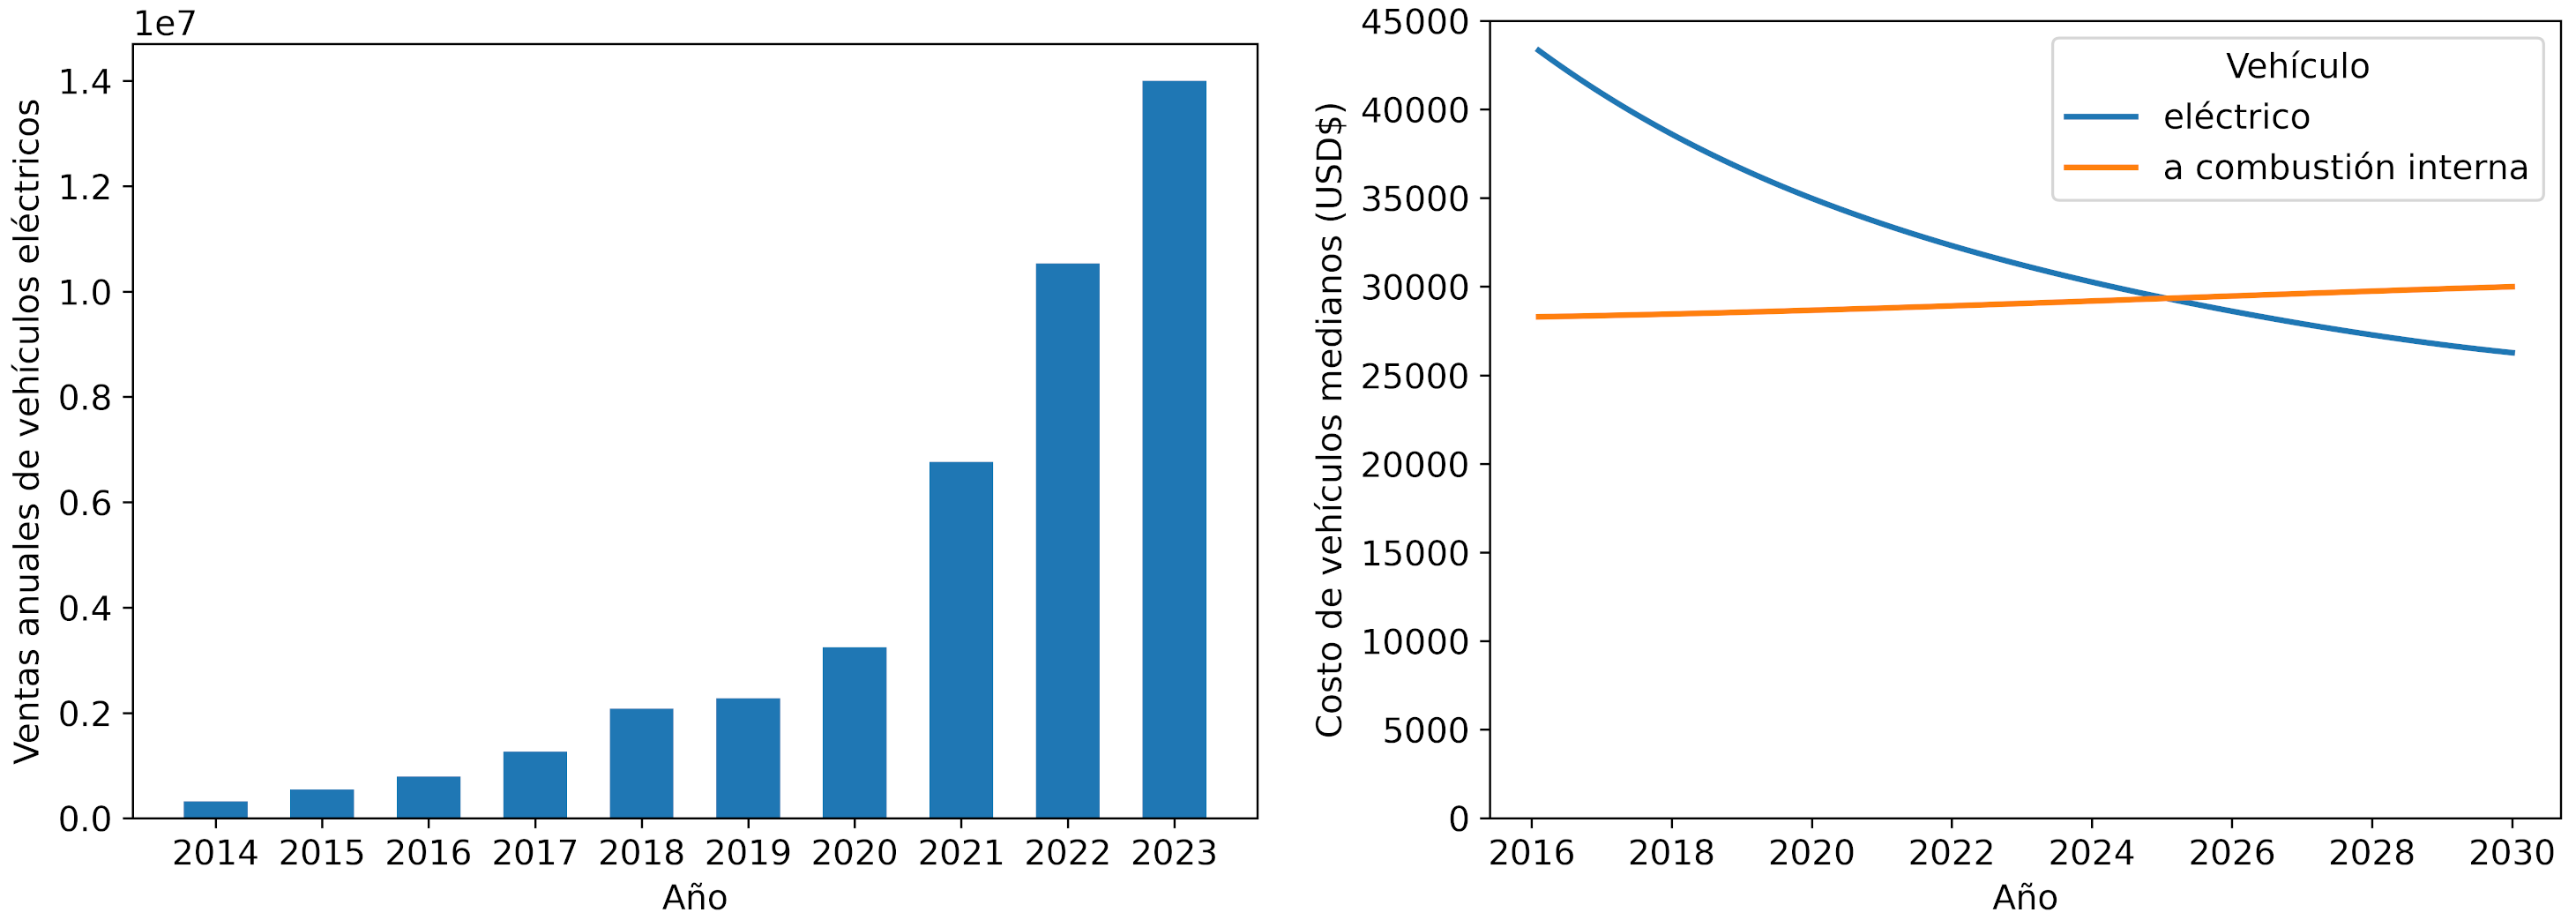
\includegraphics[width=\textwidth]{Introduccion/energia/evs.png}
    \caption{(a) Ventas anuales de vehículos eléctricos en la última década. Se 
    proyecta que para el 2030 las ventas asciendan a las 40 millones de unidades 
    frente a las 3 millones del año 2020 \cite{EVV}. (b) Proyección del costo en 
    dólares de vehículos eléctricos y de combustión interna en países 
    desarrollados \cite{BLOOMBERG}.}
    \label{fig:evs}
\end{figure}

En la Figura \ref{fig:evs}b se muestra la proyección en el costo de los vehículos 
eléctricos y de combustión interna realizada por la empresa financiera Bloomberg 
para los países desarrollados \cite{BLOOMBERG}. Se espera que para el año 2026 
los costos se igualen y que para el 2030 los EVs sean aproximadamente un 15\% más
baratos que los vehículos de combustión interna. Este cambio se debe a la 
disminución en el precio de la producción de baterías, que actualmente representa
aproximadamente el 40\% del costo del EV.

El sector energético en Argentina depende altamente de la utilización de 
combustibles fósiles, donde la generación de energía está dominada por el gas 
natural (65\%) y le siguen las centrales hidroeléctricas (18\%), plantas nucleares
(8\%), parques eólicos (7\%) y solares (1\%) \cite{IEA}. En cuanto al potencial de 
producción de fuentes renovables, Argentina tiene una gran capacidad en sus 
fuentes eólicas y solares por desarrollar. Además, es el cuarto productor mundial más 
grande de litio, que es un mineral crítico para la manufactura de sistemas de 
almacenamiento y transporte de energía, claves para la transición energética. 
El mismo representa el 7\% de la demanda para vehículos eléctricos mientras que 
para almacenamiento en la red el porcentaje es del 10\%. Otros metales y 
minerales críticos se encuentran en la región de América Latina; por ejemplo, 
Paraguay posee la reserva más grande del mundo de titanio, Chile es el mayor 
productor de cobre, Brasil tiene las segundas reservas más grande de níquel y
hierro, las terceras de grafito y manganeso, la cuarta de aluminio y la quinta de 
fósforo, por último, Cuba se encuentra en el tercer puesto de reservas de cobalto.

En la Figura \ref{fig:iea-Li} se muestra la proyección en la demanda total de 
litio por año y por aplicación, donde la mayor contribución se encuentra para la 
utilización del mismo en vehículos eléctricos mientras que una menor contribución 
se espera en aplicaciones de sistemas de almacenamiento estacionarios y otras 
aplicaciones que incluyen dispositivos electrónicos, medicamentos, lubricantes, 
entre otras \cite{IEA}. Cabe destacar que para el almacenamiento estacionario 
las baterías de ion-litio es muy probable que compitan con baterías de sodio o magnesio, entre 
otras. En el histograma de la Figura \ref{fig:iea-Li} pueden diferenciarse dos 
regiones, la primera de ellas entre el año 2022 y el 2035, donde los aumentos
porcentuales de la demanda de litio con respecto a 5 años atrás son del 74\%, 
99\% y 76\%. Luego, del año 2035 al 2040, el cambio se encuentra en el 32\% y
dicho aumento porcentual continúa disminuyendo al 10\% y al 3\% en los períodos 
subsiguientes.
\begin{figure}[h!]
    \centering
    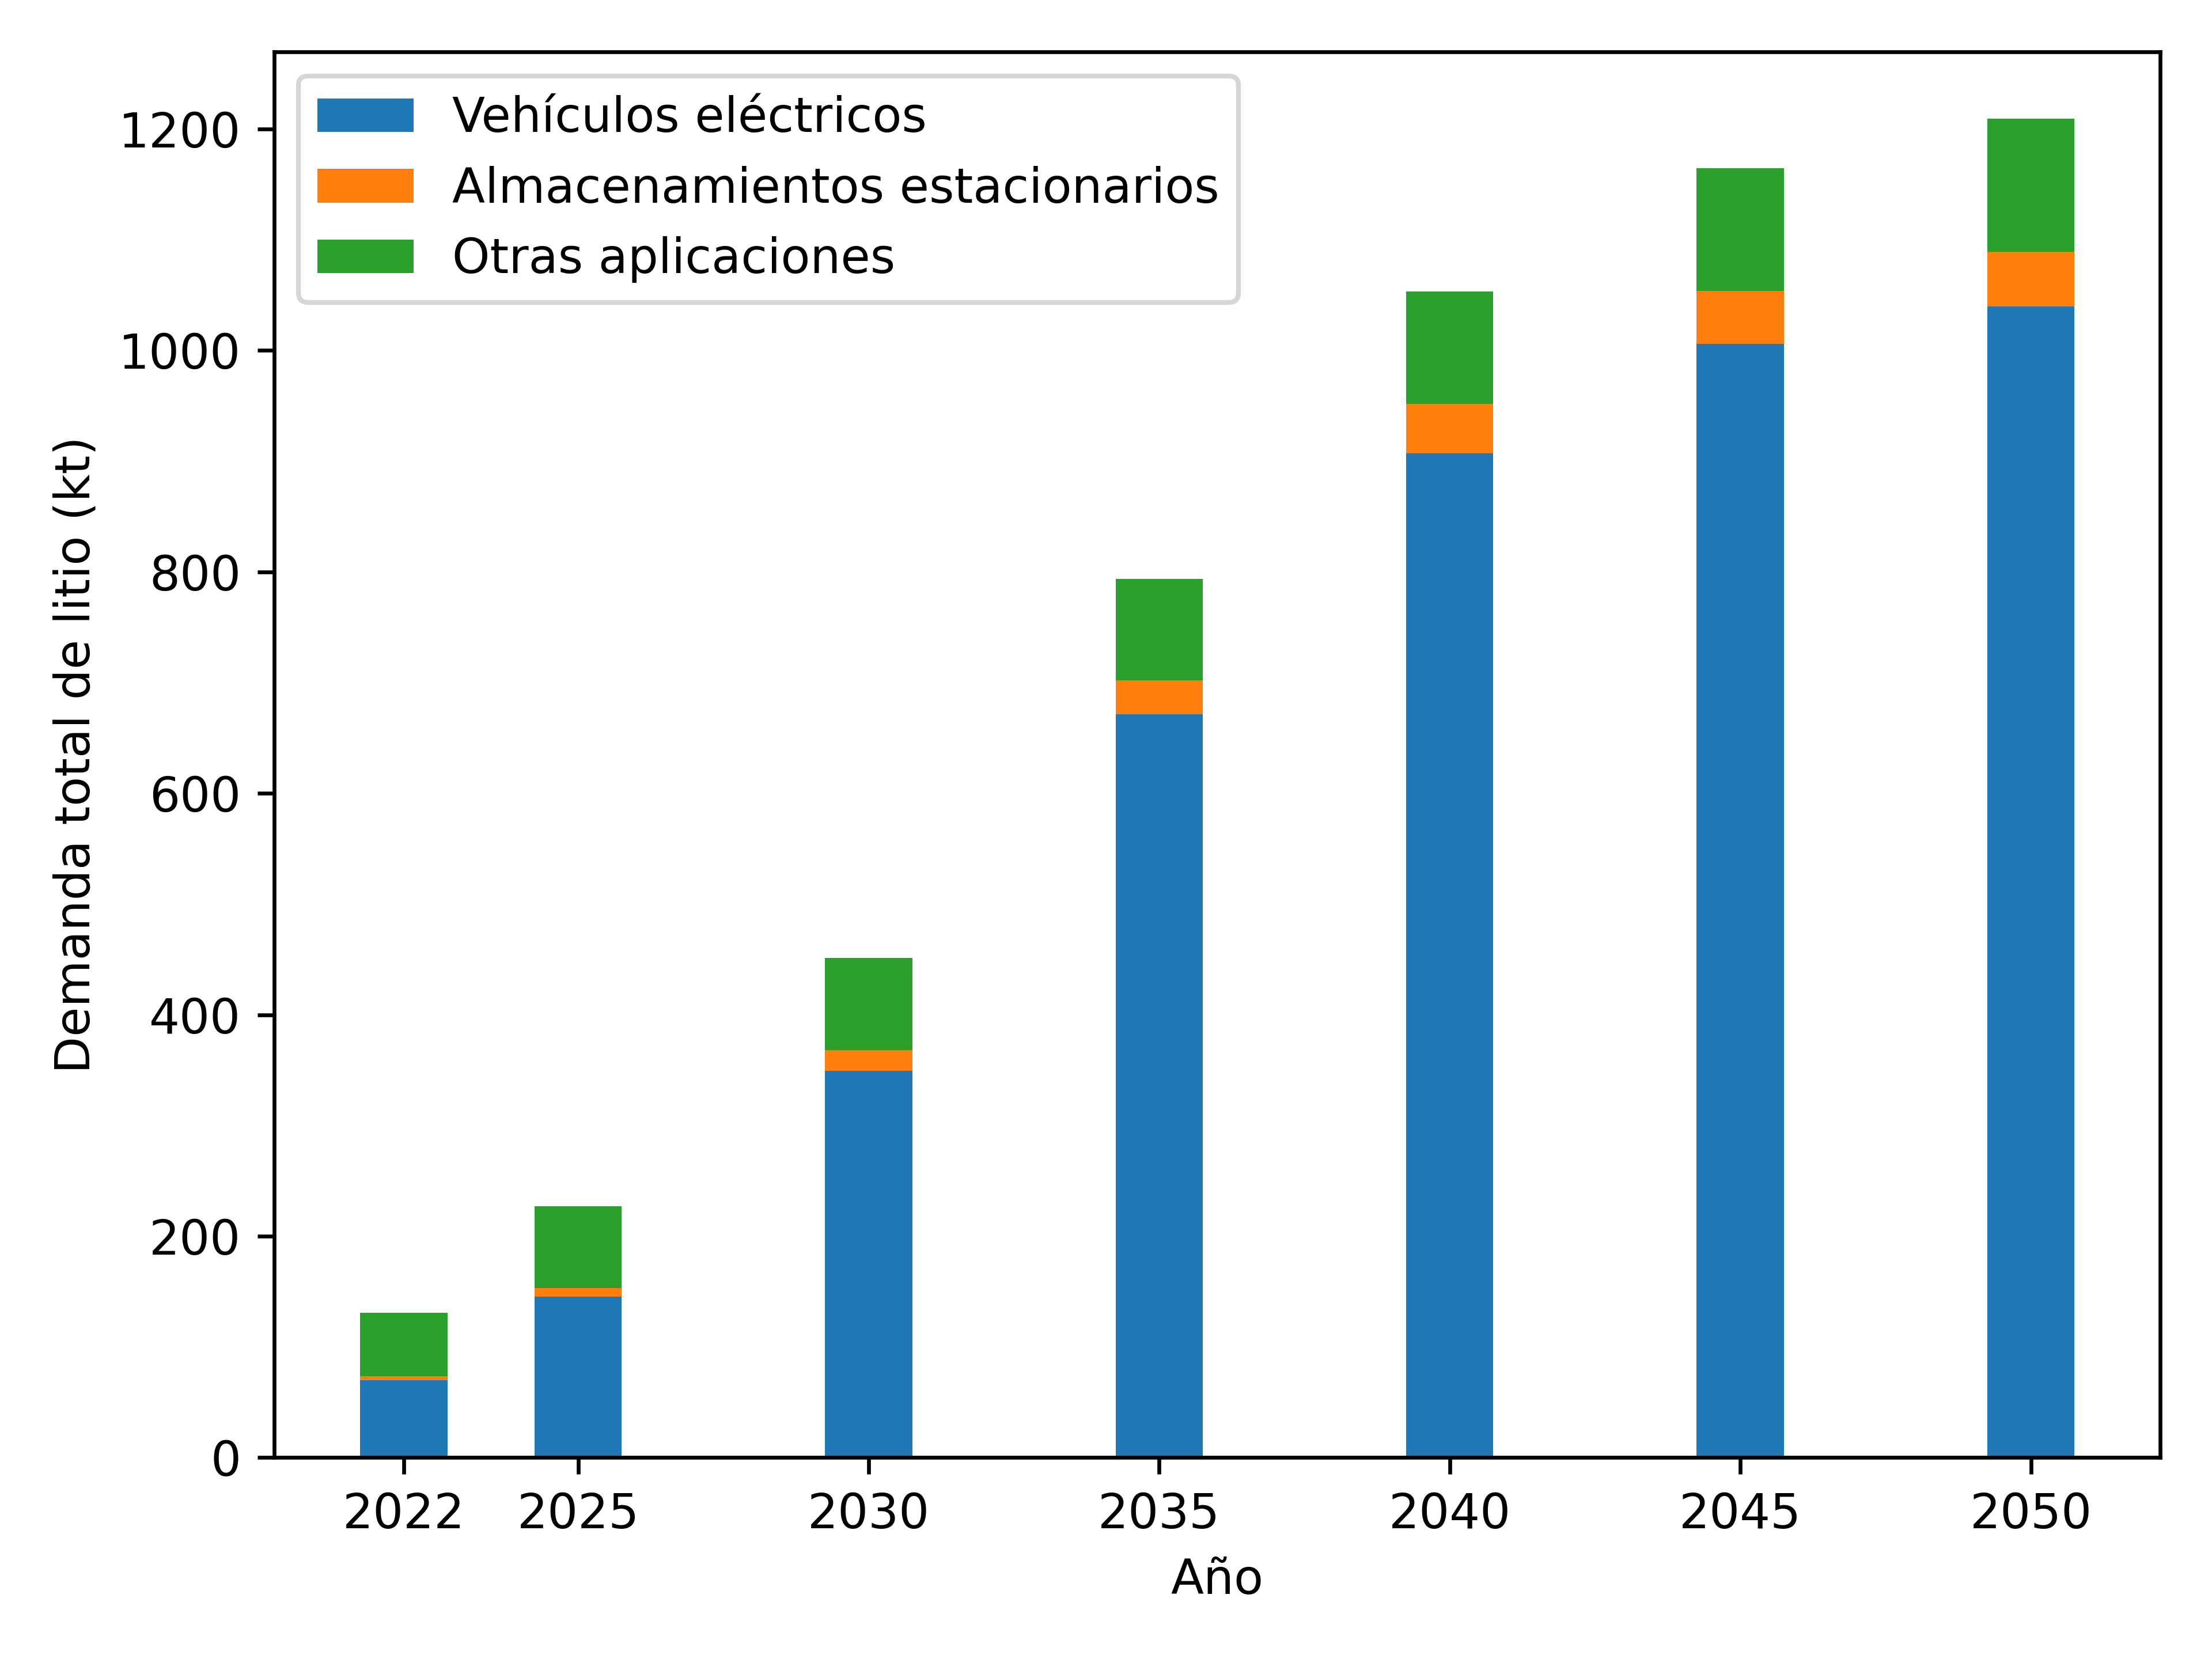
\includegraphics[width=.8\textwidth]{Introduccion/energia/iea-Li.png}
    \caption{Proyección de la demanda total de litio en kilotoneladas para el 
    período 2025-2050 para sus distintas aplicaciones: vehículos eléctricos (en 
    azul), sistemas de almacenamiento de energía estacionarios (en naranja) y
    otras aplicaciones (en verde). Fuente: \cite{IEA}.}
    \label{fig:iea-Li}
\end{figure}


\section{Baterías de ion-litio}

A finales del año 2019, año en el que se comenzó esta tesis, la Real Academia 
de Ciencias de Suecia le otorgó el Premio Nobel en Química a J. B. Goodenough, 
M. S. Whittingham y A. Yoshino por sus contribuciones al desarrollo de la batería 
de ion-litio. Esta batería recargable permitió los avances que se vieron en los 
teléfonos móviles y en las computadoras portátiles, entre otras aplicaciones.
Además, permite un mundo libre de combustibles fósiles ya que se utiliza en 
vehículos eléctricos y en almacenamientos estacionarios de energía para fuentes
renovables. Este galardón restaltó la importancia de muchos aspectos de la ciencia
moderna, como la investigación básica, la investigación la aplicada, la 
interdisciplina (JBG fue físico, MSW es un químico y AY un ingeniero) los 
desarrollos tecnológicos y los problemas concretos de las sociedades.
En la década del 1970, MSW desarrolló la primera batería utilizando un ánodo de
litio metálico y un cátodo de disulfuro de titanio. En 1980, JBG duplicó el 
voltaje original de dicha batería al introducir un cátodo de óxido de cobalto.
La desventaja de ambas se encontraba en el ánodo de litio metálico, que en los 
ciclos de carga y descarga se deposita preferentemente en sitios donde ya se 
ha depositado, dando lugar a estructuras ramificadas, llamadas dendritas, que 
pueden cortocircuitar la celda y llevar a la explosión de la misma. En 1985,
AY remplazó este material por uno carbonoso que incorpora los iones de litio
durante la carga y la descarga, disminuyendo los riesgos mencionados. Basandose
en este desarrolló, Sony comenzó a comercializar baterías de ion-litio en 1991.
La densidad de energía de estas baterías rondaba los 80 Wh/kg, en la actualidad
WeLion comercializa para los EVs de Nio una batería de ion-litio con una 
densidad de energía de 360 Wh/kg. En la Figura \ref{fig:whkg} se muestra la 
evolución de la densidad de energía en baterías de ion-litio comercializadas 
en los últimos 30 años. La importancia de esta característica para los EVs 
radica en la relación autonomía/peso.
\begin{figure}[h!]
    \centering
    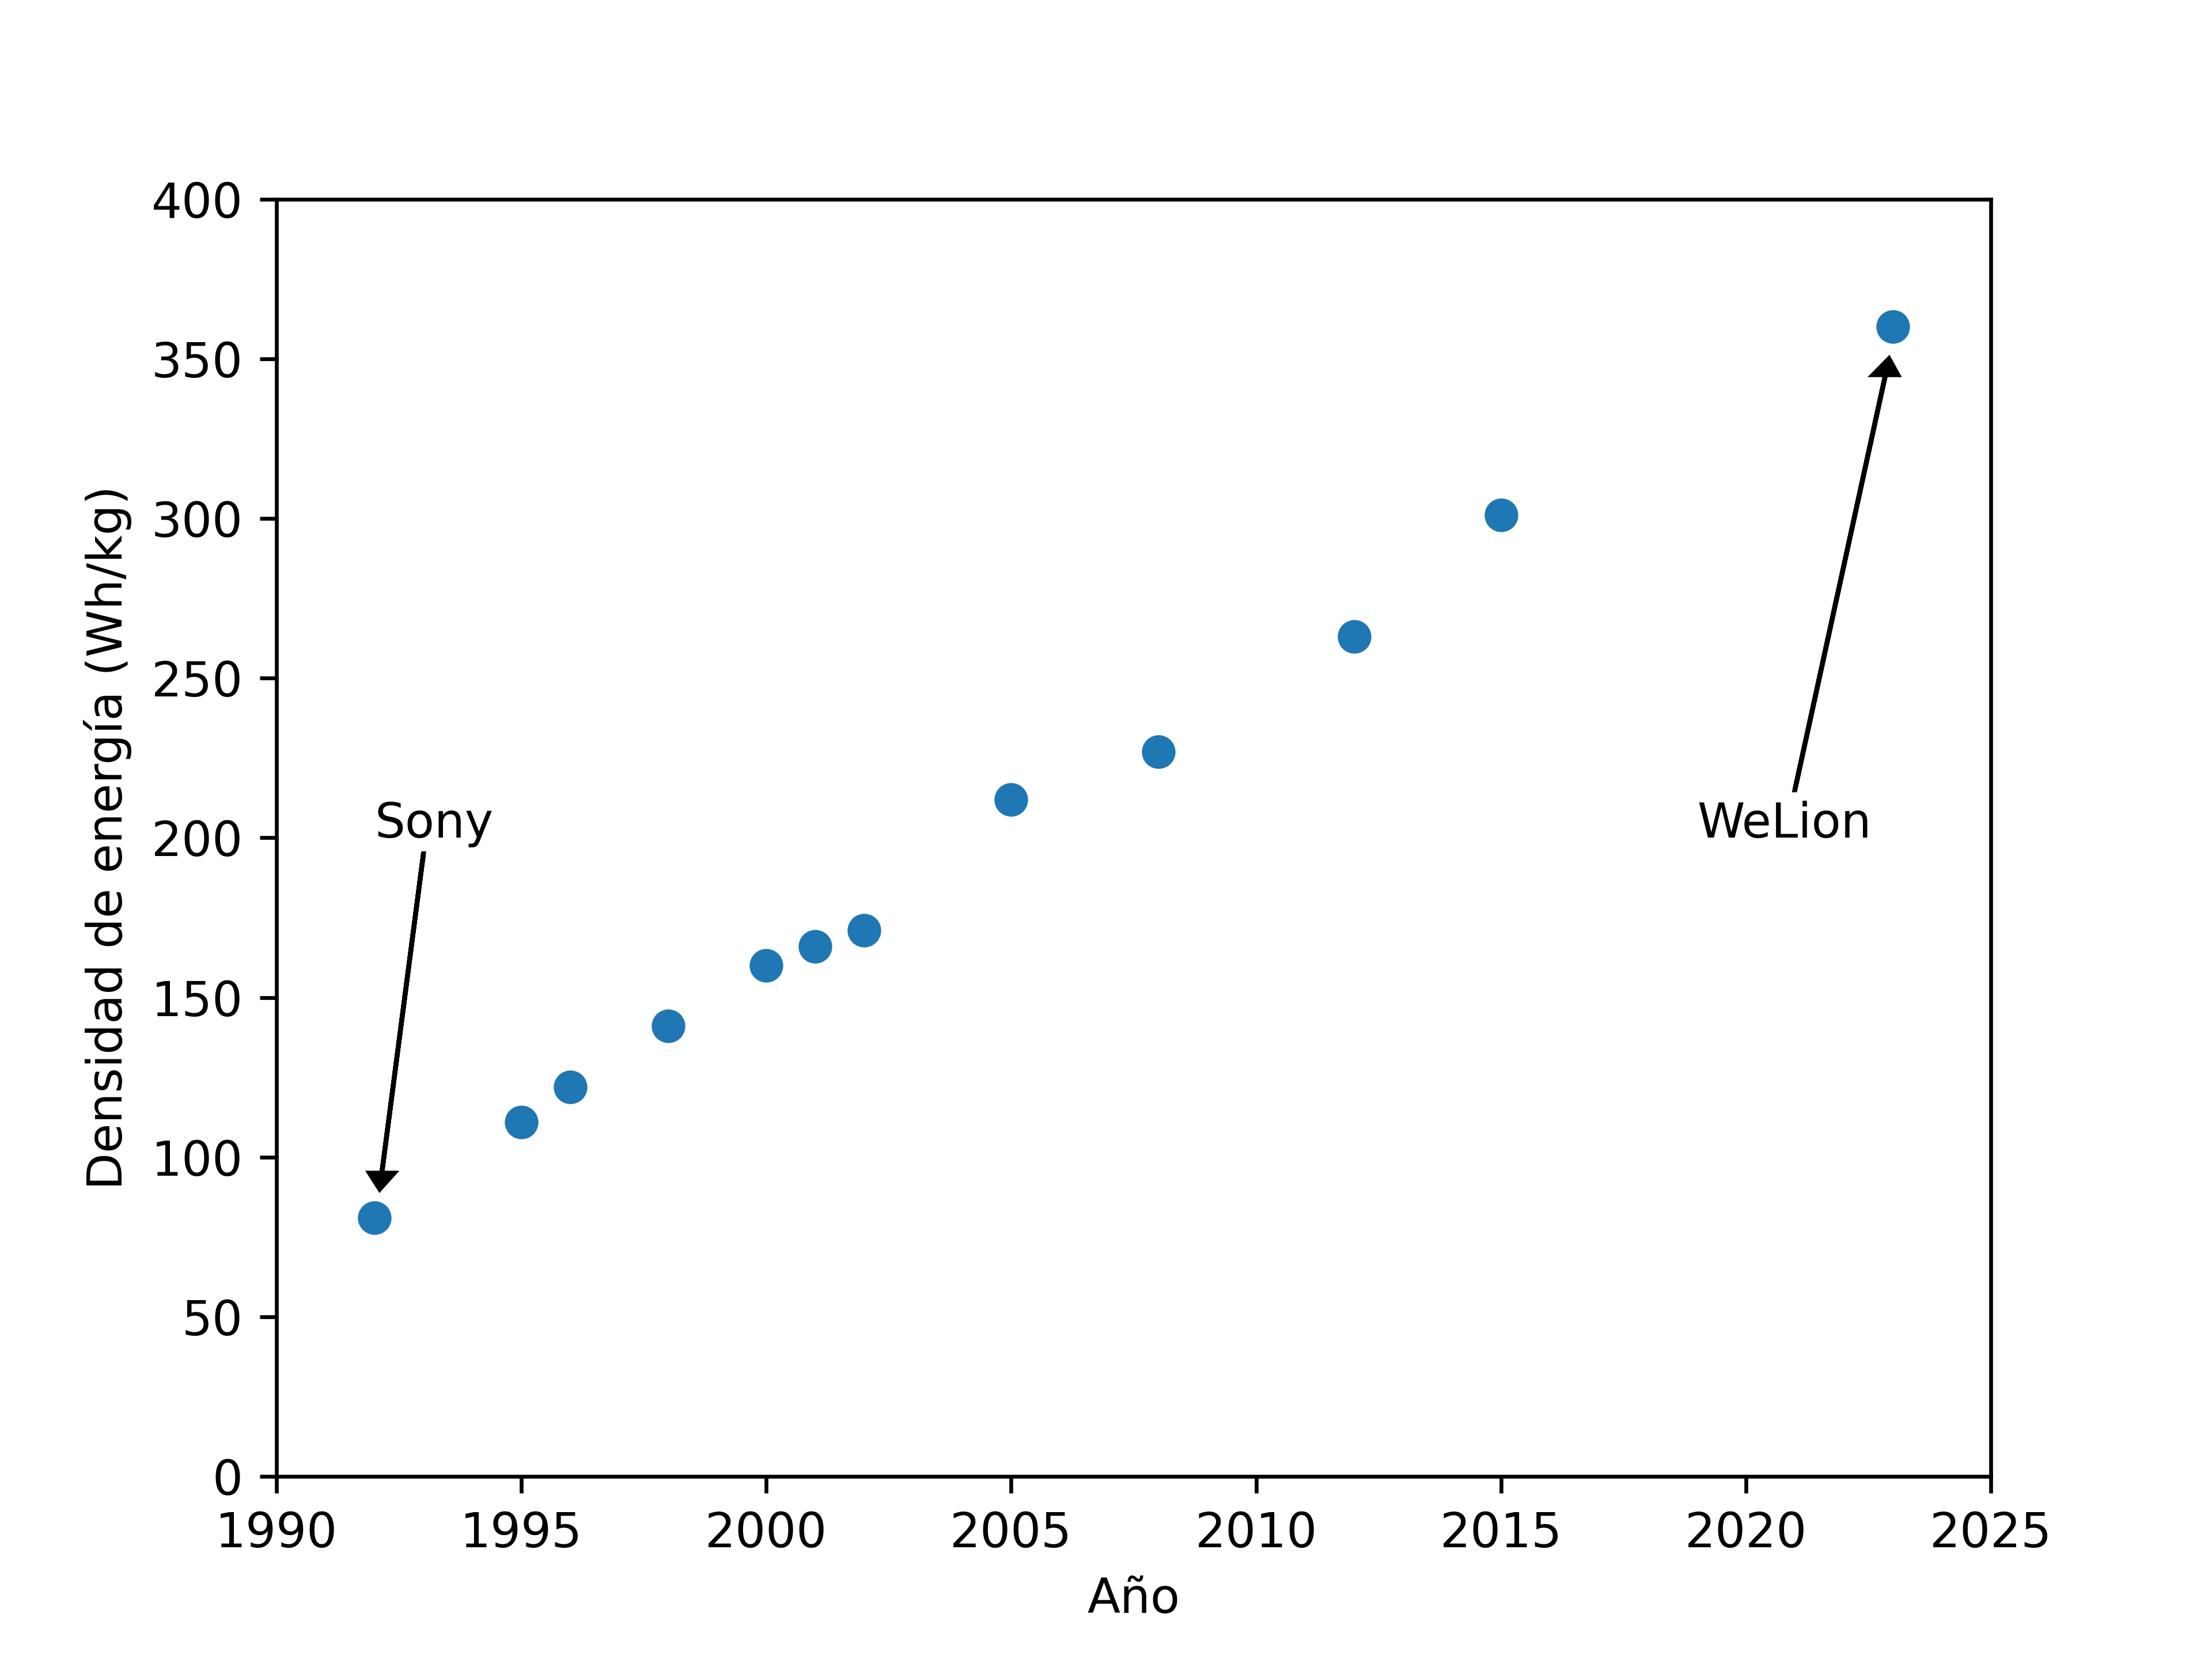
\includegraphics[width=.8\textwidth]{Introduccion/baterias/whkg.png}
    \caption{Aumento en la densidad de energía en baterías de ion-litio comercializadas
    en los últimos 30 años. Figura adaptada de \cite{li2023700}.}
    \label{fig:whkg}
\end{figure}

Las baterías de ion-litio admiten una gran cantidad de recargas y las mismas están 
compuestas por celdas electroquímicas conectadas entre sí, las mismas son unidades 
fundamentales que permiten transformar la energía química almacenada en energía
eléctrica mediante una reacción redox (reducción-oxidación), en la cual uno de los 
componentes pierde electrones (se oxida) y el otro gana electrones (se reduce).
En la Figura \ref{fig:esquema_bateria} se muestra un esquema general con el 
funcionamiento que presenta una celda electroquímica de ion-litio y se destacan 
las componentes más relevantes: los electrodos positivo (cátodo) y negativo (ánodo) 
donde ocurren las reacciones redox en la carga/descarga de la celda, el electrolito 
por el cual difunden los iones de litio y el separador que suele ser un material 
poroso permeable al electrolito que se encarga de que los electrones circulen por 
el circuito externo. Durante la descarga de la reacción redox es espontánea y 
provoca la difusión de iones de litio por el electrolito desde el ánodo hacia el 
cátodo, junto con una corriente eléctrica en un circuito externo (flechas rojas). 
Durante la carga se debe aplicar una corriente eléctrica externa para tener la 
reacción inversa (flechas verdes).
\begin{figure}[h!]
    \centering
    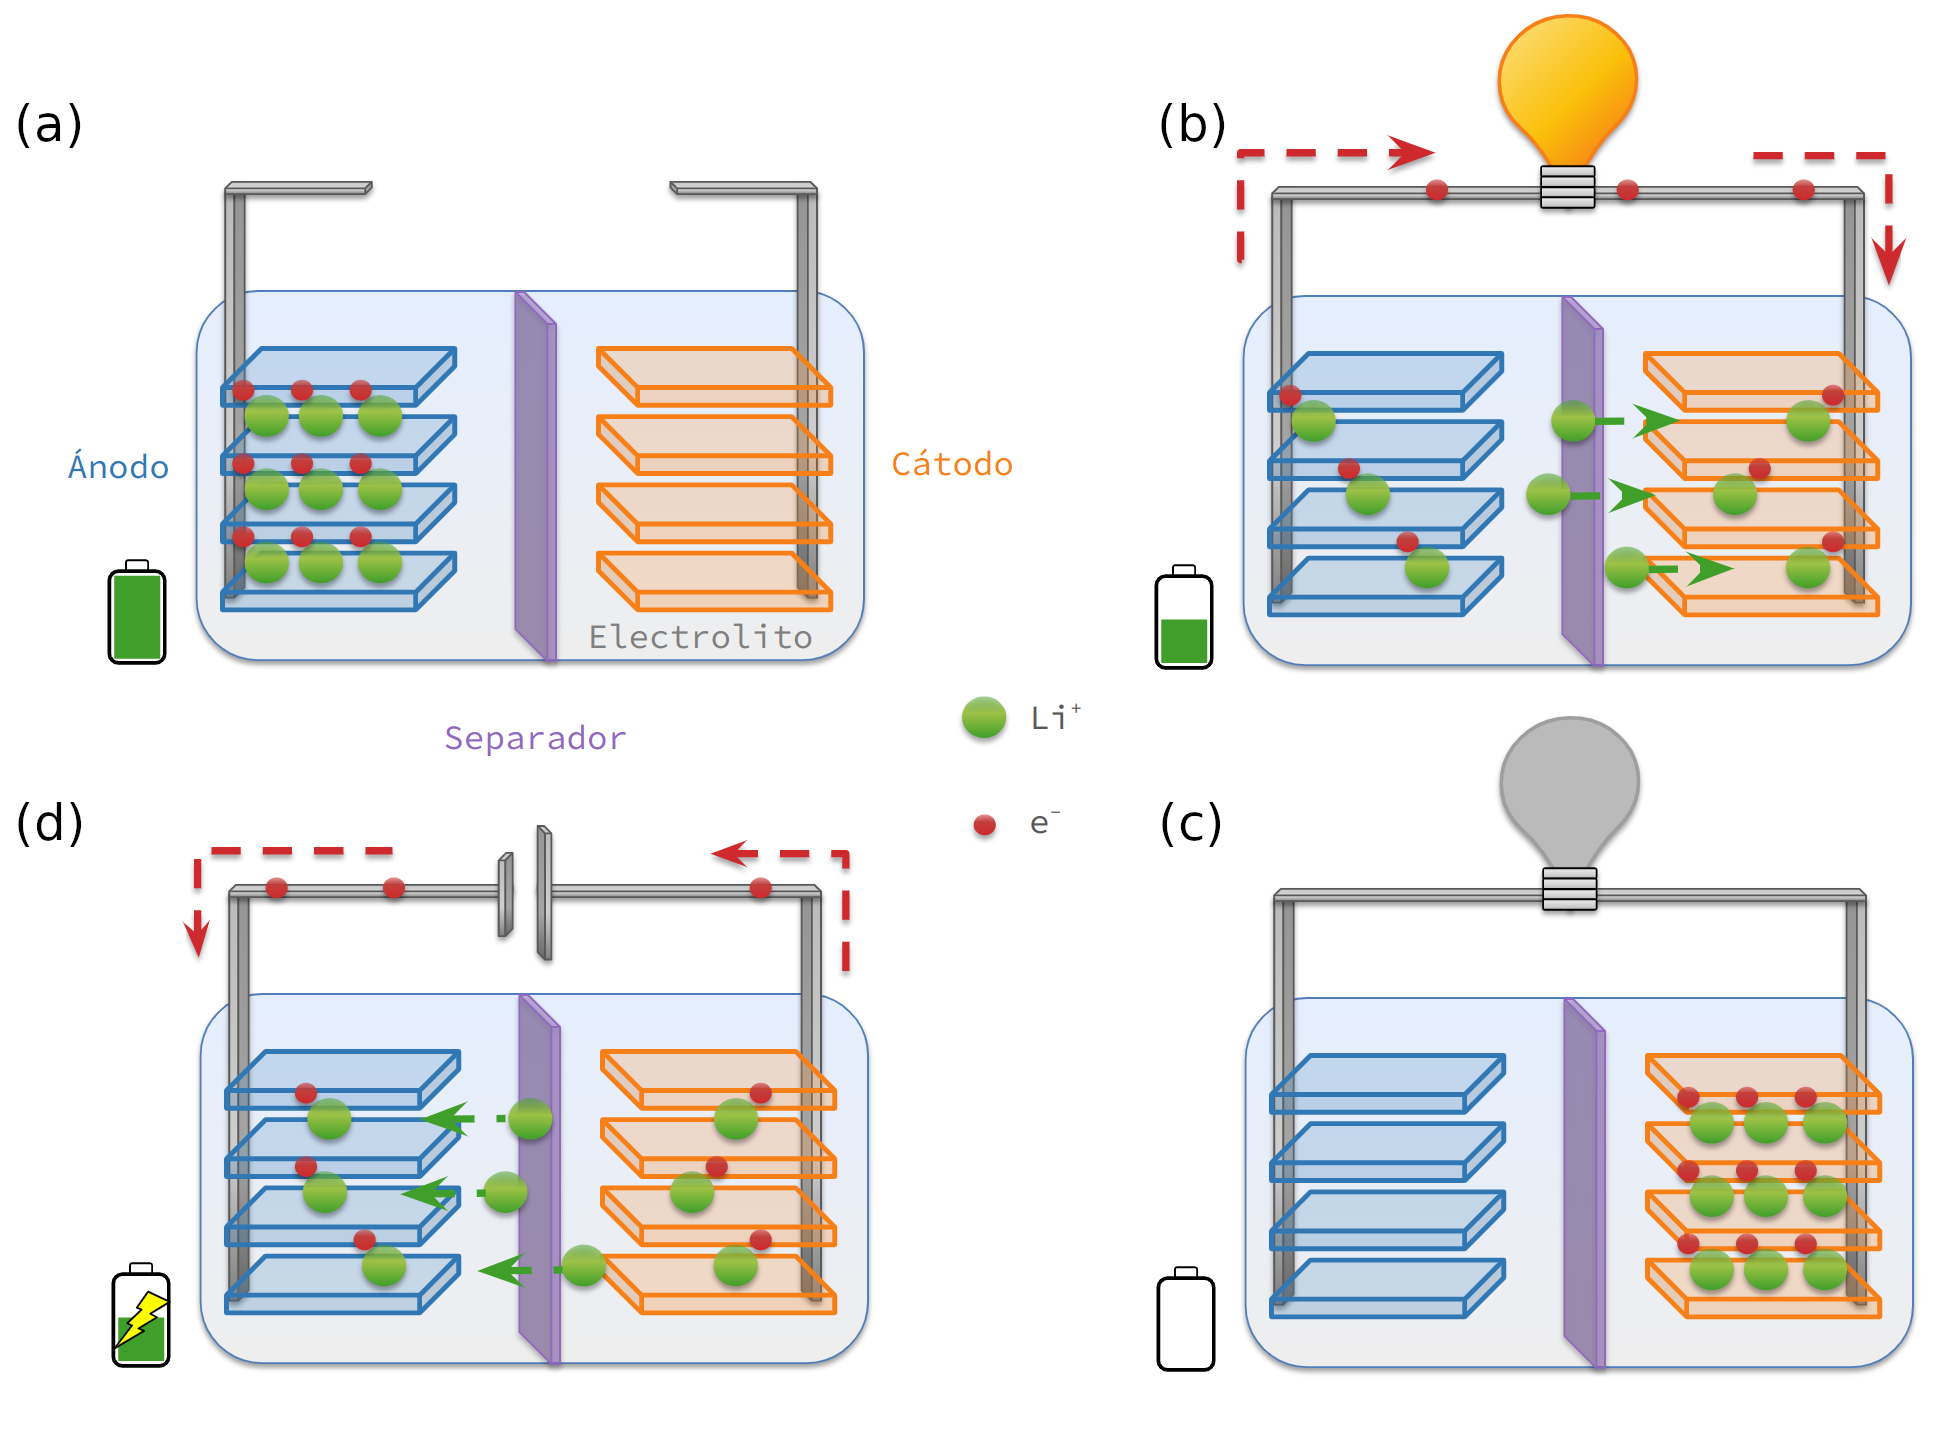
\includegraphics[width=.8\textwidth]{Introduccion/baterias/esquema_bateria.png}
    \caption{Esquema de las componentes y el funcionamiento de una batería de 
    ion-litio.}
    \label{fig:esquema-bateria}
\end{figure}

En la Figura \ref{fig:scopus} se muestra el incremento en las últimas dos décadas
de los artículos científicos publicados en el área de las baterías de litio y, en 
particular, de las dos ramas estudiadas en esta tesis: la Carga rápida y los 
Ánodos de Si. En dicha figura se presentan datos extraídos de la base de datos 
Scopus \cite{SCOPUS} del número de publicaciones anuales normalizado con respecto 
al número de publicaciones en el año 2003, año en el que hubo 710 publicaciones 
en baterías de litio, 32 sobre ánodos de Si y 0 sobre carga rápida, por lo que 
se normalizó en este caso a la única publicación del 2004 en el tema.
\begin{figure}[h!]
    \centering
    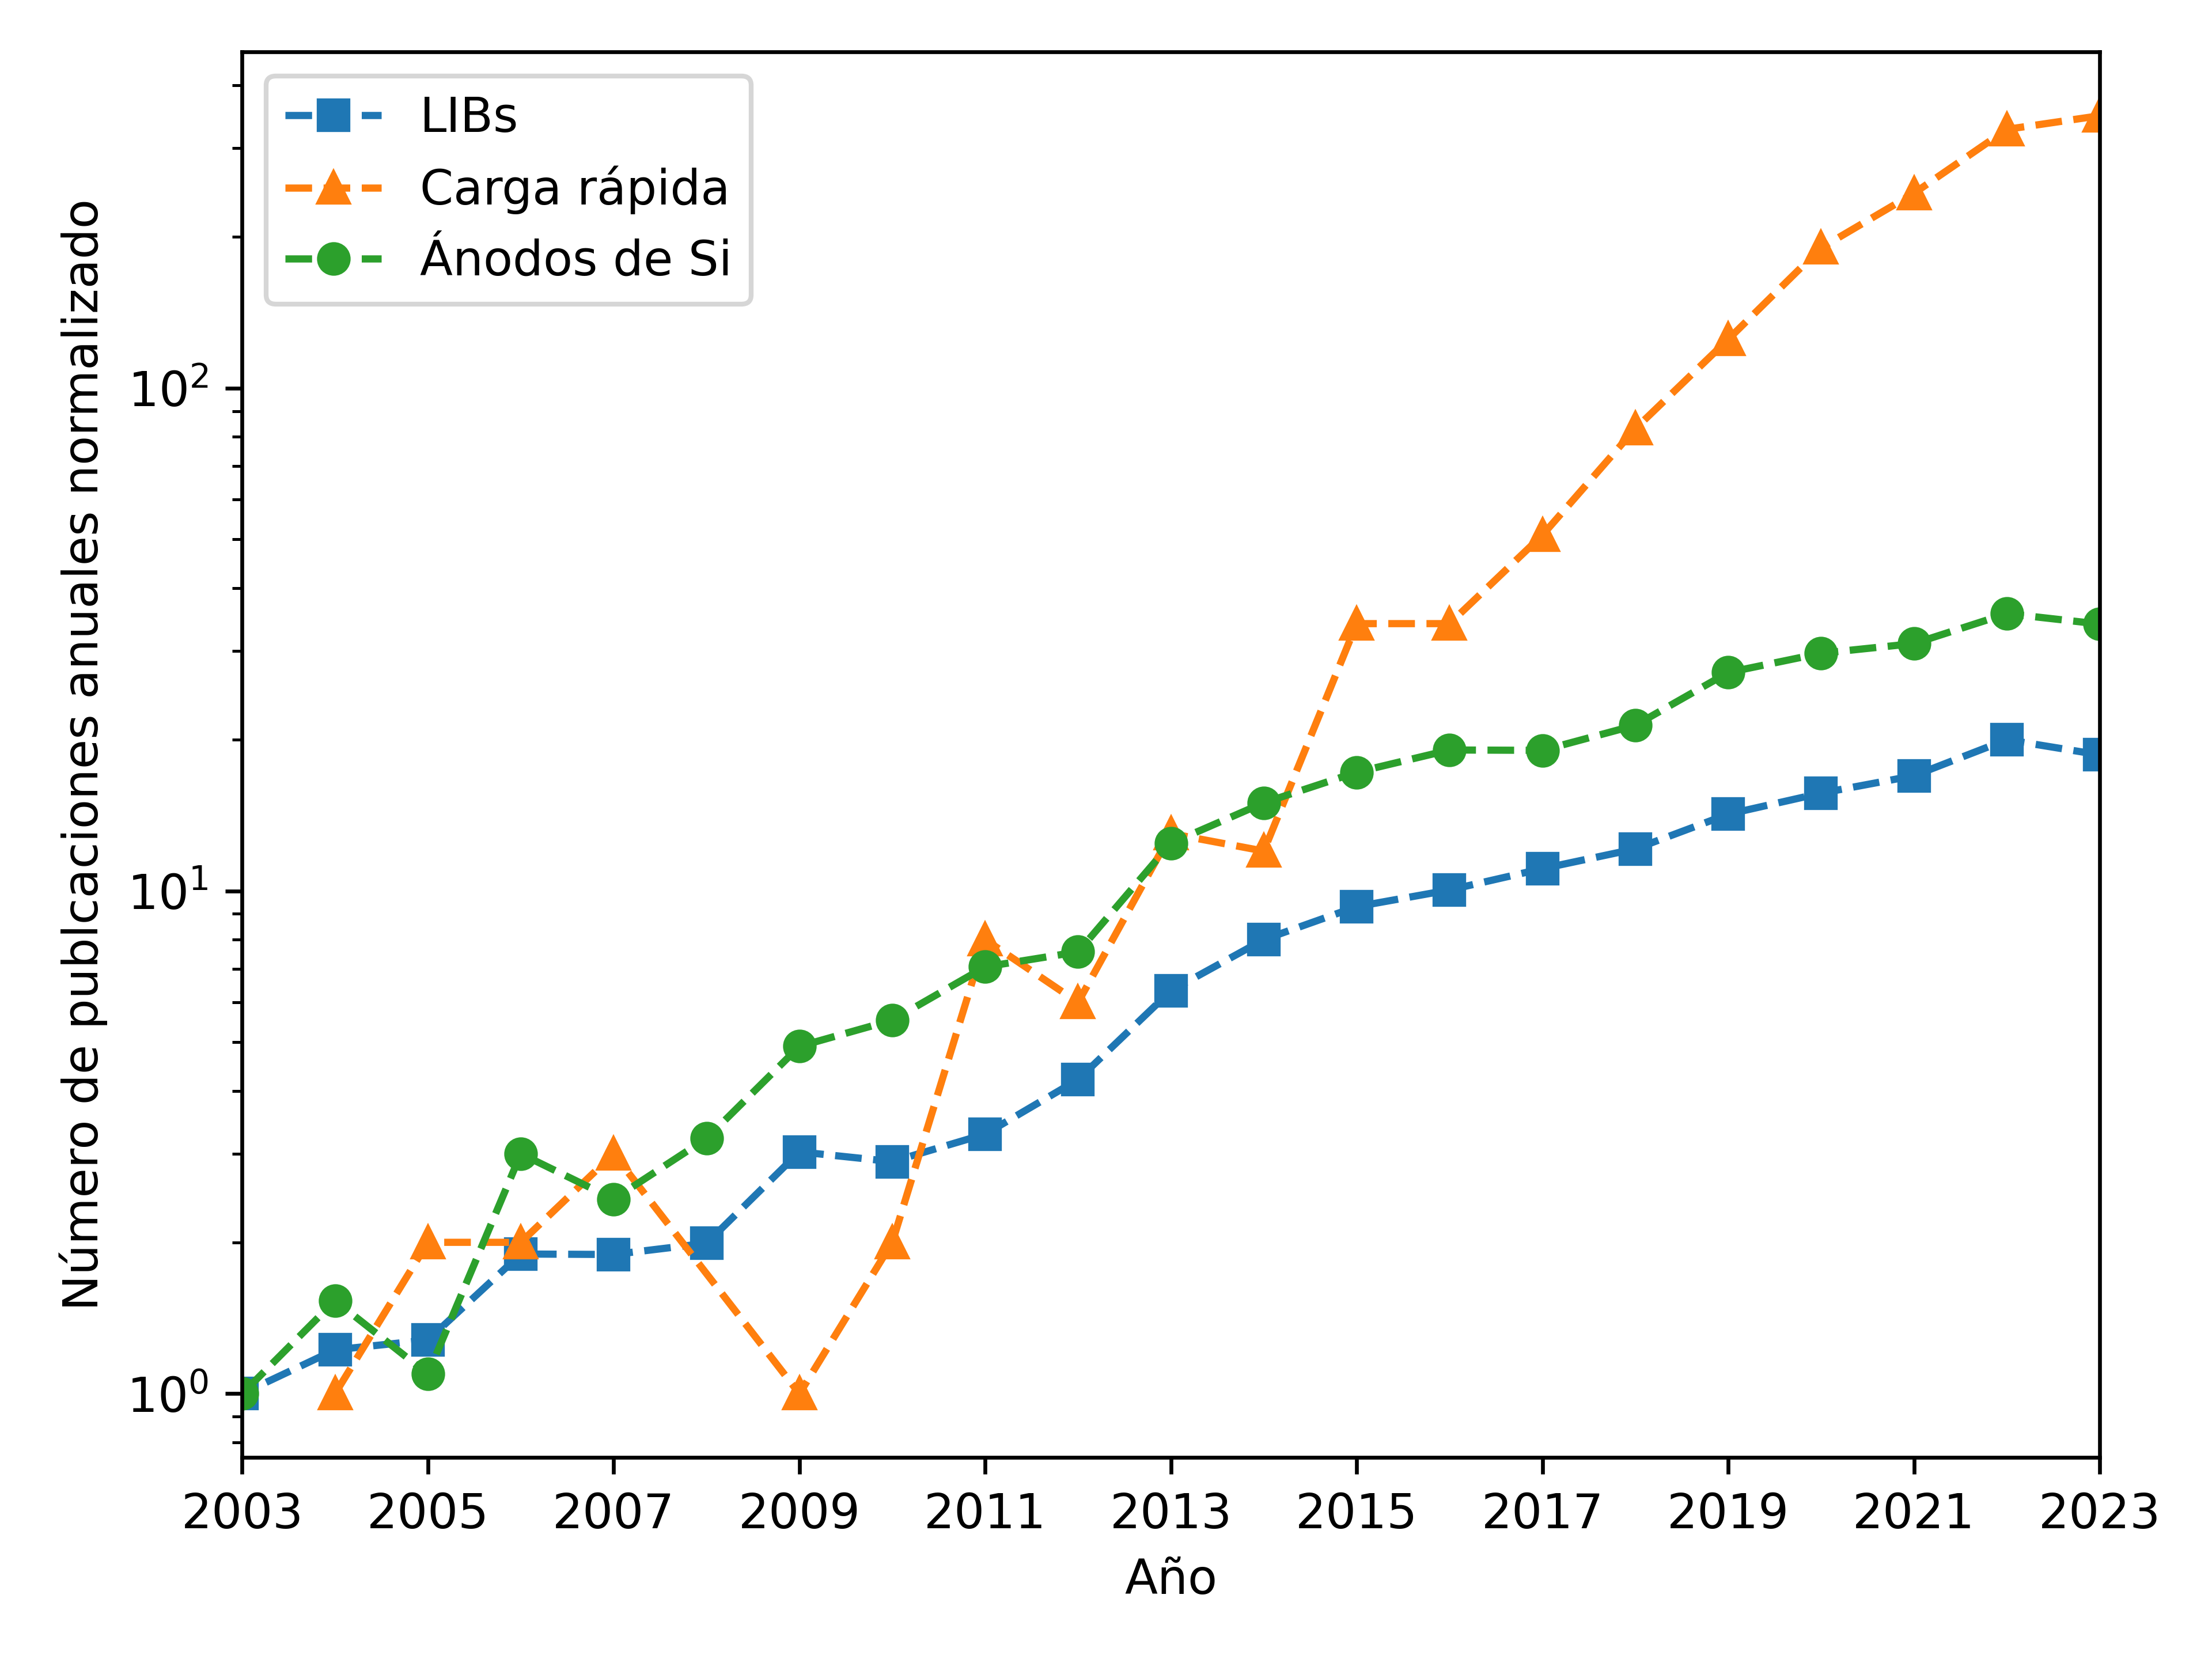
\includegraphics[width=.8\textwidth]{Introduccion/baterias/scopus.png}
    \caption{Número de publicaciones anuales normalizado con respecto al año 2003. 
    Las consultas realizadas en Scopus \cite{SCOPUS} incluyen: 
    \texttt{lithium AND battery} (LIBs, en azul), \texttt{lithium AND battery AND 
    fast-charging} (Carga rápida, en naranja) y \texttt{lithium AND battery AND 
    silicon anodes} (Ánodos de Si, en verde).}
    \label{fig:scopus}
\end{figure}
La normalización y la escala logarítmica en la Figura \ref{fig:scopus} permiten
observar cualitativamente que la pendiente de crecimiento de publicaciones 
realcionadas a la carga rápida de baterías de litio es considerablemente mayor a 
de las otras dos. Además, los ánodos de Si se encuentran dentro de lo que sería
el creciemiento promedio del área de las baterías de litio. Un análisis de datos
cuantitativo permite determinar que en la última década el aumento de porcentaje
anual de publicaciones promedio fue del 15 \% y 16 \% para las baterías de litio 
y para los ánodos de silicio, respectivamente, mientras que para la carga rápida 
este porcentaje promedio asciende al 52 \%. Este análisis demuestra la relevancia
que la comunidad científica le da a los temas estudiados en esta tesis.


\section{Objetivos y estructura de la tesis}

Esta tesis tiene como objetivo estudiar materiales que se utilicen para el 
desarrollo de electrodos de baterías de ion-litio de próxima generación mediante 
distintos modelados computacionales. 
La misma se encuentra dividida en tres partes, la primera de ellas sobre la 
Motivación y fundamentos consistente de dos capítulos, el capítulo 
\ref{ch:introduccion} con esta introducción y el capítulo \ref{ch:metodos} con la
descripción de los distintos métodos computacionales utilizados. 
La Parte \ref{p:fast-charging} se divide en dos capítulos, ambos relacionados con 
la carga rápida de baterías de ion-litio. En el capítulo \ref{ch:un} se 
desarrolla un modelo para ajustar datos experimentales en condiciones 
galvanostáticas y predecir el tamaño óptimo de partículas que permita retener un 
80 \% de su capacidad frente a una carga realizada en 15 minutos 
\cite{fernandez2023towards}. El capítulo \ref{ch:umbem} introduce por primera vez en la literatura una métrica 
universal que permite estandarizar las comparaciones del desempeño entre 
distintos materiales considerados en aplicaciones de carga rápida.
La Parte \ref{p:silicio} se centra en el estudio de las aleaciones presentes en 
los ánodos de silicio y se divide en tres capítulos. El capítulo 
\ref{ch:caracterizacion} caracteriza las estructuras de Li-Si encontradas con 
un potencial reactivo y con un método de exploración acelerada de mínimos locales
propuesto \cite{fernandez2021characterization}. En el capítulo \ref{ch:modelo} se
parametriza un modelo DFTB (\textit{denstity functional tight-binding}) para la 
interacción Li-Si mediante un algoritmo que asigna pesos a las distintas 
estructuras consideradas para el ajuste \cite{oviedo2023}. En el capítulo 
\ref{ch:prediccion} se proponen modelos de vecinos más cercanos para predecir 
mediciones de rayos x, RMN y Mössbauer a partir de las configuraciones atómicas
\cite{fernandez2023nmr}.
Cada uno de los capítulos mencionados en estas dos últimas partes se componen
de una introducción, detalles de los métodos computacionales utilizados, los 
resultados junto a las discusiones de los mismos y conclusiones parciales.
Por último, se cierra la tesis con el capítulo \ref{ch:comentarios} con los 
comentarios finales de la misma.

